\chapter{Theoretical Foundations } \label{cap:teoria}
  
In this chapter a quick review of the main characteristics of time series, as well as of Neural Networks, especially those that will be applied to the problem of interest, called Multilayer Perceptron Networks (MLP) and Gated Recurrent Unit (GRU).  

    \section{Demand Forecasting Methods} 
    
Demand forecasting can be defined as a process of searching for information that produces sales of a product or a set of products.

        In \citeonline{moreira1998} are defined as methods of demand forecasting that use such information to estimate future demand, and can fit this definition from subjective and intuitive methods to mathematical and computational methods. In the same article, the forecast models are classified into two major groups: qualitative methods and quantitative methods.
        
         In  \citeonline{Junior2007} has been made the evaluation of several methods of demand forecasting, which are schematized in the Figure  \ref{fig: metodosPrevisaoDemanda}. 
        
                  \begin{figure}[ht]
                  	\center{
                  	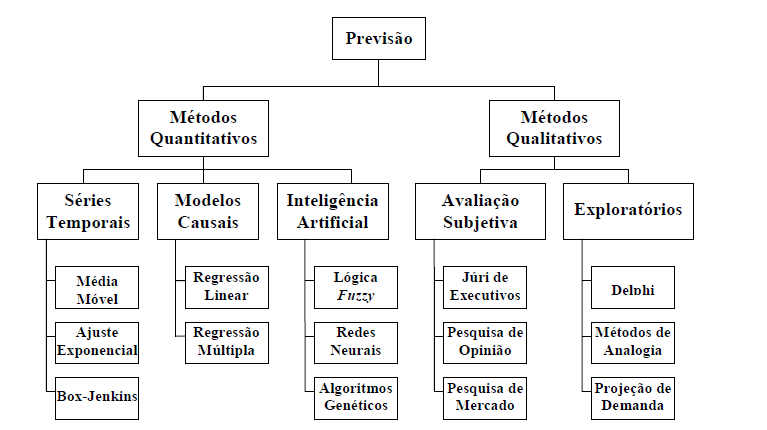
\includegraphics[width=\textwidth]{./Figs/01-junior-metodos-previsao-demanda.png}
                  	\caption{Demand forecasting methods.}\caption*{  Source: \cite{Junior2007}.}
                  	\label{fig: metodosPrevisaoDemanda}}
                  \end{figure}
        
        Quality methods are defined in \cite{Junior2007} as a judgment of the data exposed without processing analytics, such as grouping and classification of data. These methods do not provide new numerical information or predict models.
        
        On the other hand, quantitative methods are defined, in the same study, as being analytical and based on mathematical models for performing predictions. These methods analyze behavior patterns from a data historical, aiming to predict future behavior.
         
        In \citeonline{Junior2007} is also mentioned that the data collected for forecasting models, when graphically projected, show behaviors that can be generalized in a subjective way by managers of the data. For all cases, data analysis is necessary to select the parameters of the demand to make objective predictions.  Yet, only data analysis may be insufficient, and if performed with incorrect criteria it may compromise the conclusions of the studies. 
        
         Data analysis is a large process that aims to treat data from its acquisition and pre-processing until its interpretation using complex mining tools. In different steps, diverse mathematical, probabilistic, statistical, computational and heuristic techniques are involved.  In Section \ref{sec: timeseries} will be commented the main characteristics of the time series, which will be the forecasting method applied to the practical problem of interest. 
    
        \subsection{Time Series} \label{sec: timeseries} 
         
            According to \citeonline{Morettin1987}, a temporal series is a set of observations ordered in function of time, commonly the same, presenting a serial dependence among itself. Also it can be defined as a realization of a set of random variables  $ X=\{x_1, x_2, \dots, x_T\}$, ordered in time, where  $T$ represents the length of the series, as is made in \cite{defts}. The correlation between the variables is usually described by their collective distribution function or in other cases by the media and covariances. 
            
            Among the objectives of time series analysis, the following can be emphasized: i) describe the behavior of the series identifying trends and variations, ii) analyze and mold the dependency between the observations, and iii) fmake forecasts of future series values. 
            
            Time series have a deterministic component and a random component, they can be continuous or discrete, depending on the type of observation of the variables. They are called stationary when the properties of mean, variance and covariance are kept in time. The trend references the rate of growth or decrease, and can be linear, exponential or cushioned. Yet the oscillation of the trend is known as the cycle. In addition, they can present seasonality, in other words, exhibit behavior that has a tendency to repeat itself in a certain number of time periods.
    
             Examples of each of these properties, as well as techniques applied to study and correct each of them can be seen in \cite{tecnicas1}. These features, together with the random component study, provide information of interest for practical applications.
             
            %\TODOR{Passar pra metodologia ou literatura, não falar do trabalho aqui}
            Because of the objective of this work, temporal series will be applied for events with seasonality in order to estimate forecasts. The techniques to do this are using regression methods and some practical applications can be seen to include forecasting of realized power consumption, as made in \citeonline{Almeida2013}, \citeonline{RUAS2012} and \citeonline{Silva2010}, and of the demand forecast of cosmetic products, as it can be seen on\citeonline{Junior2007}.
    
    \section{Artificial Neural Networks}
    
        Artificial Neural Networks are tools with multidisciplinary basis, once they are nourished by knowledge of neuroscience, mathematics, statistics, physics, computer science and engineering \cite{Haykin1994}, and are part of the great area of knowledge called Artificial Intelligence (AI), term pointed out in \cite{kaplan2019siri}.
        
        In a nutshell, it could be defined that "artificial intelligence is the branch of computer science that deals with intelligent behavior. \cite{Luger2004}. Artificial Intelligence systems seek to solve functions and problems inspired by two human characteristics: the capacity for abstraction and learning from the error.
        
        In the context of Artificial Intelligence, a neuron is a unit considered fundamental for information processing, and Neural Networks are sets of artificial neurons interconnected through connections, logical and mathematical functions \cite{Haykin1994}. Neurons of a network are capable of processing multiple values of inputs and react quickly producing a related response to these inputs, simulating the behavior of the human brain. 
        
        Inspired by a search for a computational model of the biological neuron, the first artificial neuron model, called MCP, was proposed in the article \textit{ A Logical Calculus of the Ideas Immanent in Nervous Activity.} \cite{mcculloch43a}, an illustration adapted for \cite{lemos} of this model can be found in the figure \ref{fig: NeuronioArtificial}.
        
        McCuloch was a psychiatrist and neuroanatomist and spent about 20 years reflecting and studying about the representation of the nervous system, in 1942 he invited Pitts who was a mathematician to be part of his researches.
        
        The structure of the artificial neuron reacts to an input vector and synapses are represented by numerical weights. A transfer function also called the activation function, measures a linear combination of the input values and the synapses weights, determining if or not the neuron is activated depending on the value obtained. If the neuron is activated an output value of 1 is emitted, otherwise an output value of 0 is emitted.
            \begin{figure}[ht]
                \center{
                  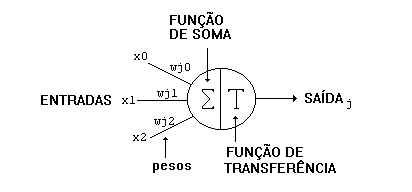
\includegraphics[width=0.65\textwidth]
                  {./Figs/02-neuronio-artificial.png}
                \caption{Artificial Neuron. }\caption*{  Source: \cite{lemos}} \label{fig: NeuronioArtificial} }
            \end{figure}
            
        The whole functionality of this model is then reduced to reply if the weighted sum received is greater than an established numerical value. Although, associated to this neuron was not proposed an automatic way to adjust the weights, that means no learning algorithm was given to train the neuron. This problem was later solved by Perceptron's formulation.
        
        In \citeonline{Haykin1994} in Chapter 1.9 entitled \textit{Historical Notes}, is introduced in more detail the fascinating history of the development of Neural Networks from the initial conception of biological neuron studies until complex networks of supervised learning known as \textit{Vector Support Machines}.
            
        \subsection{Perceptron} \label{sec: perceptron}
    
            The proposed neuron model in \citeonline{mcculloch43a}, even though it simulated a biological neuron and solved some logical and mathematical tasks, it did not satisfy the main objective of Artificial Intelligence: The capacity of learning. To be able to use this structure, it was necessary to know how to adjust the weights of the inputs, which was not a trivial problem in many cases. 
                        
            The first neuron with a learning algorithm was suggested in \citeonline{perceptron} and was named Perceptron. In this study, the weights of the connections are adjusted autonomously with the introduction of associated weights and a Bias value, in order to search for an autonomous recognition of standards. In the figure \ref{fig: perceptron} a schematic of the operation of the structure is presented.
            
            \begin{figure}[ht]
            	\center{
              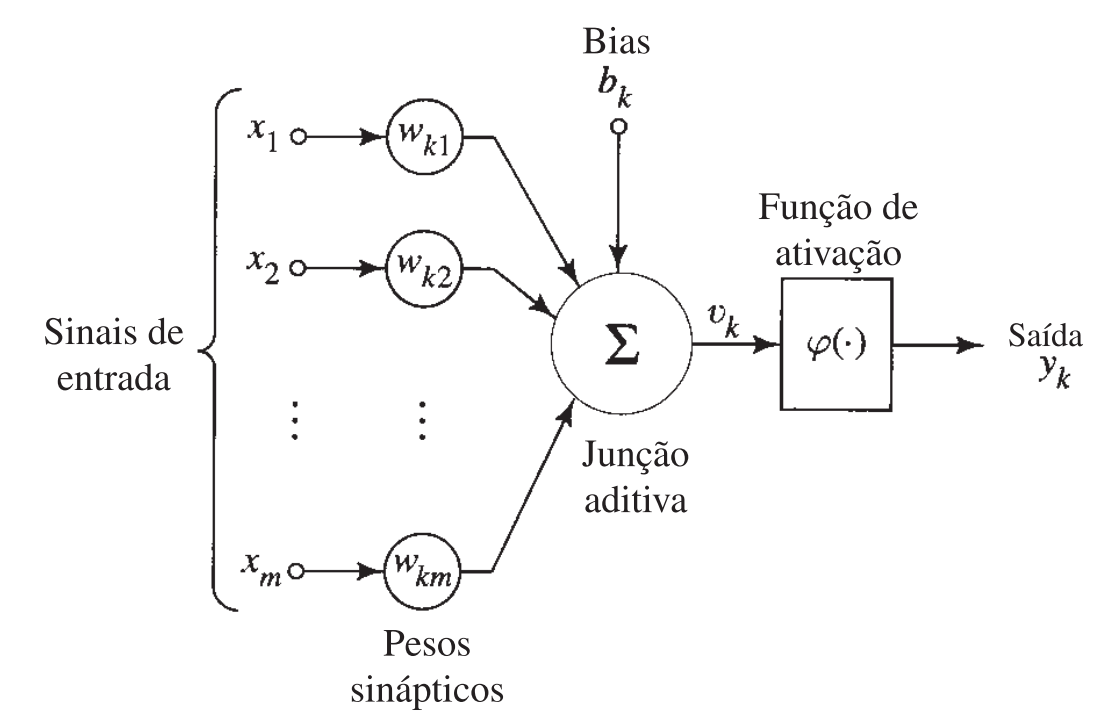
\includegraphics[width=0.65\textwidth]
              {./Figs/03-perceptron.png}
            \caption{Artificial Neuron Perceptron. }\caption*{  Source: \citeonline{Haykin1994}} \label{fig: perceptron} }
            \end{figure}
            
            But in \citeonline{perceptrons2} was proven that because of the learning model limited to a linear combination, the perceptron could only solve linearly separable problems. In the figure \ref{fig:problemasLineares} two simple problems are presented, one that perceptron can solve \textit{(a)}, and another does not \textit{(b)}.
            
            \begin{figure}[ht]
              	\center{
              	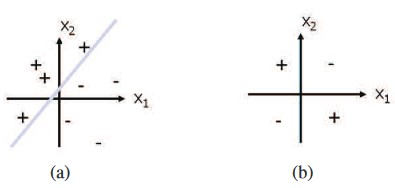
\includegraphics[width=0.8\textwidth]{./Figs/04-limite-perceptron.jpg}
              	\caption{Problem linearly separable (a) and not separable (b).}\caption*{  Source: \cite{Flavia2014}.}
              	\label{fig:problemasLineares}
              	}	
            \end{figure}
            
            Almost two decades later, it was released in \cite{rede1} the first model of a Neural Net, called a perceptron net, applying the training by linear combinations to a set of interconnected perceptrons. This approach allowed solving more complex problems through a combination of solutions. 
              
            The network had just one input layer, one output and an activation function  $ \varphi $ \cite{Haykin1994}. Perceptron network activation function could still be linear or non-linear. In the figure \ref{fig:activation_functions} some commonly used activation functions are illustrated. 
            
             \begin{figure}[ht]
                \center{
            	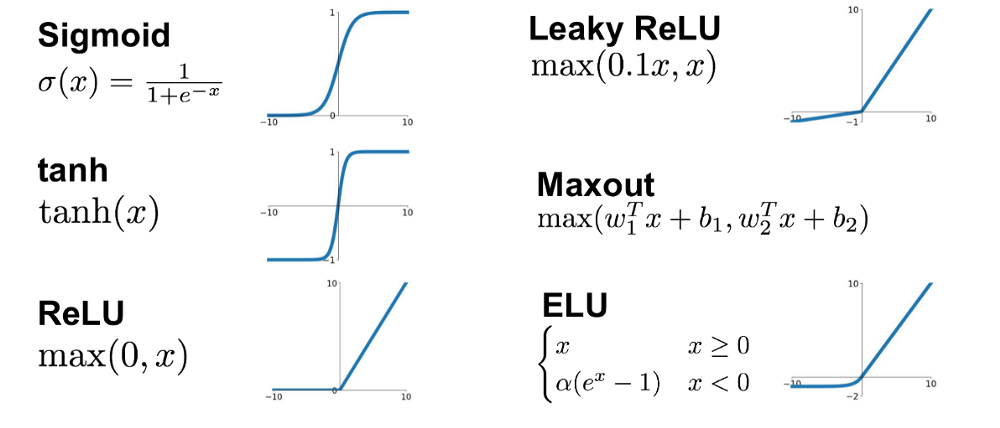
\includegraphics[width=0.80\textwidth] {./Figs/05-funcoes-ativacao.png}
                \caption{Examples of Activation functions.}\caption*{  Source: \cite{MCAI}} \label{fig:activation_functions}} 
            \end{figure}
            
            In \citeonline{Almeida2013} the learning process of the perceptron network is analyzed in a supervised way. During this process, the structure learns to relate an observed set of input variables in the network to one or more expected output values named as real values or truth values. Then the learning results are analyzed by comparing these values with the values generated by the perceptron net over the same set of data, and from this comparison is calculated the error measurement of the training.
                        
            A criterion for stopping training algorithm is to check whether the error is acceptable or not. If positive, the neural network maintains the values of the synapses weights obtained at the time. If not, a new training season is made trying to adjust the weights to obtain a smaller failure.
            The other criterion for stopping training is to reach a maximum number of training periods allowed. The adjustment of weights is called the rate of learning.
            
            The next step in developing Neural Network models is related to the topology that determines the amount of perceptrons in the network and how they connect, generating multi-layered networks.        
    
        \subsection{MultiLayer Network Perceptron (MLP)}
    
            The possibility of combining two or more layers of perceptrons was given by the use of an output signal combiner perceptron. With it the Neural Networks are scaled up to several interconnected perceptrons columns. Each column is denominated a hidden layer of the Neural Network. The last layer must have the number of perceptrons corresponding to the number of desired outputs. In the figure \ref{fig:MLP} a Neural Network with 2 hidden layers is presented, whose output layer has 3 neurons.
            
            \begin{figure}[ht]
             \center{
             	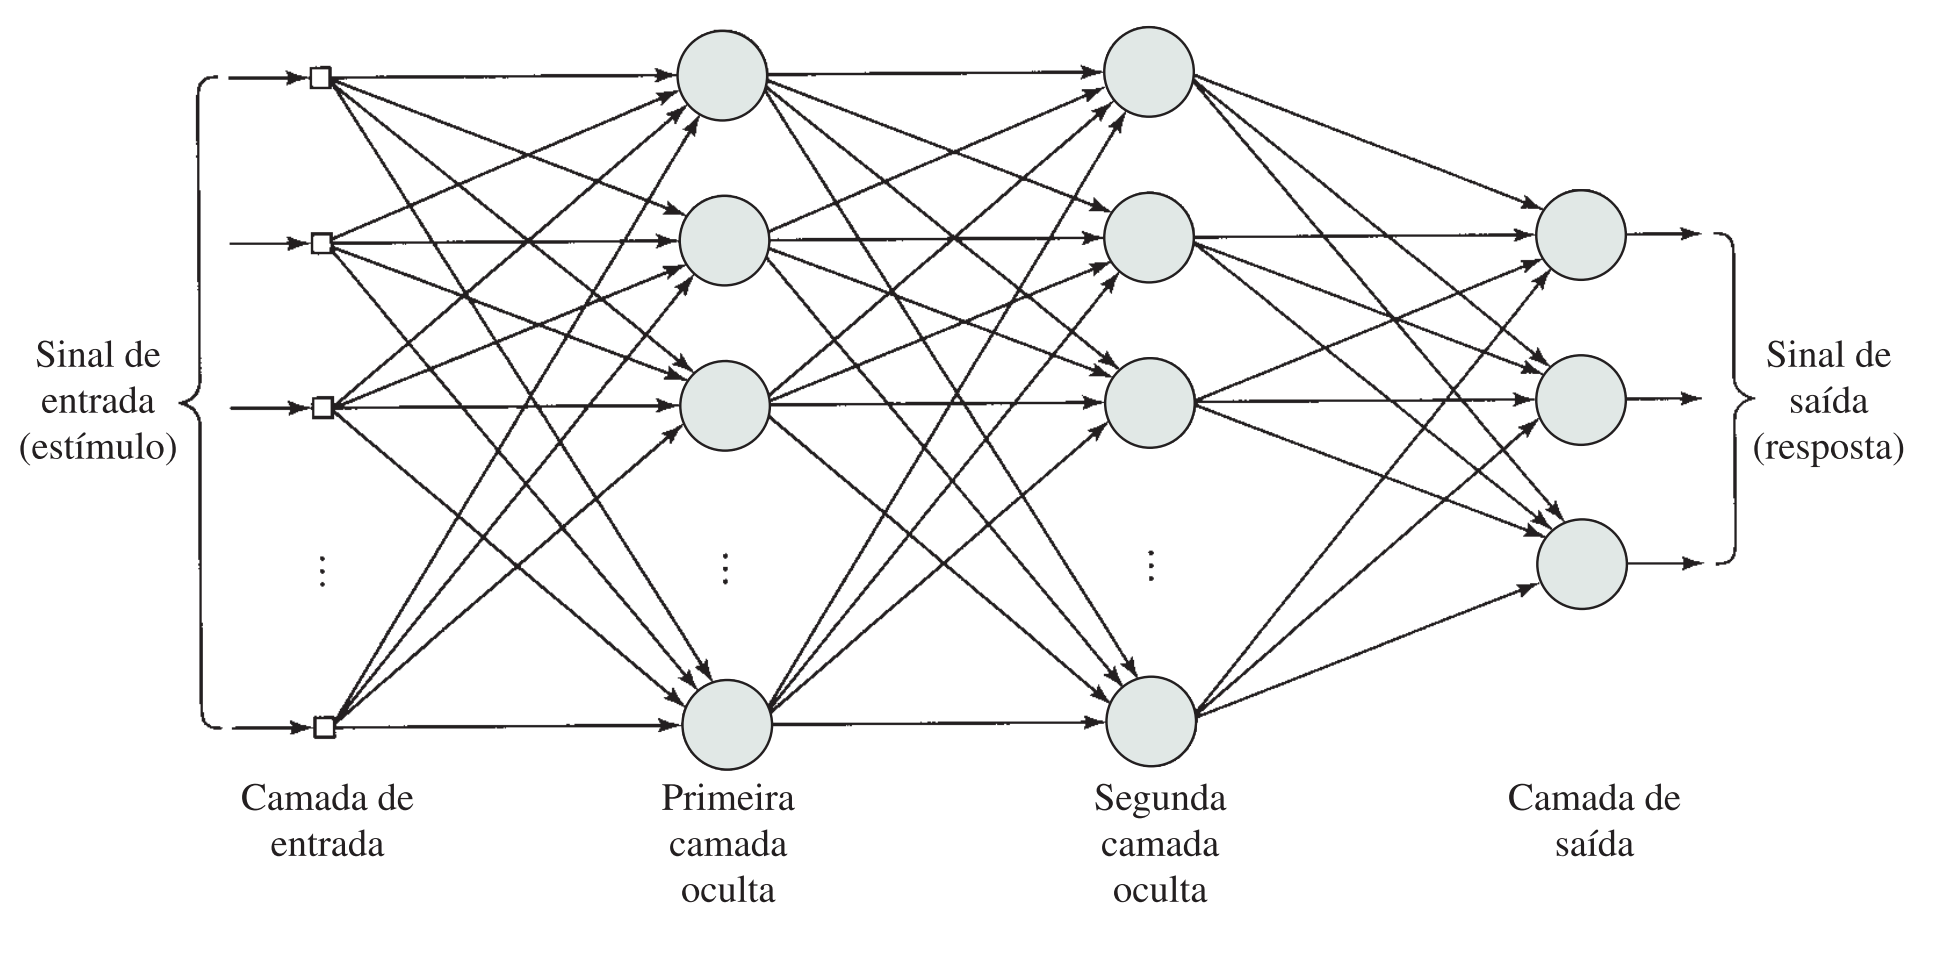
\includegraphics[width=\textwidth]
             	{./Figs/06-MLP.PNG}
             \caption{MultiLayer Network Perceptron. }\caption*{  Source: \cite{Haykin1994}\label{fig:MLP}
             }}
            \end{figure}
            
            In \citeonline{Braga2000} is postulated that through an intermediate layer it is possible to approximate any continuous function and further that two intermediate layers are enough to approximate any mathematical function. If the use of two or more layers can facilitate the training of the network, it becomes unviable to use a large number of these, since in each hidden layer the error is estimated from the error in the previous layer, which generates loss of accuracy.
            
            In practical applications, it has been seen that in some cases, the capacity for abstraction and recognition of Neural Network patterns overcome human capabilities. In other cases a network may not produce an expected response by incorrectly solving a problem, as well as the human brain, because of learning limitations or training failures. 
              
            To train an MLP network in a supervised way, the input data set must be divided into two subsets, one of \textit{training} and another of \textit{validation}. These subsets can be separated with various techniques. Thus, for example in \citeonline{DLB} a heuristic form of set separation in random order is presented, with 70\% of the data for training and 30\% of the data for validation.
            
            About the maximum number of training attempts allowed, very long training sessions tend to memorize weights of the values observed in the training data.  This implies a loss of network generalization capacity, resulting in a difficulty to evaluate entries outside the training data. This phenomenon is known as \textit{overfitting}.
            
            There is also another way of training an MLP network, called cross-validation, which was presented in \cite{crossvalidation}. This technique consists of exchanging the sets of training and validation at different times of training. In that case, the measurement of the validation error goes through an evaluation process taking into consideration the number of periods. By evaluating the average quadratic error of both sets it is possible to detect the beginning of the \textit{overfitting}. For this reason, the optimal stopping point of the training is associated with the lower limit of this mean square error in the validation set illustrated in the figure \ref{fig:validacaoCruzada} as an early stopping point for \textit{overfitting}.
            
            \begin{figure}[ht]
              \center{
              	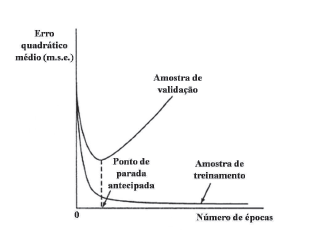
\includegraphics[width=0.5\textwidth]
              	{./Figs/07-validacaocruzada.png}
              
              \caption{Ideal stop point of cross validation. }\caption*{ Source: \cite{Haykin1994}} \label{fig:validacaoCruzada}} 
            \end{figure}
    
        \subsection{Multiple Layer Perceptron Network with \textit{Backpropagation}.}
    
            The learning method for multi-layered Neural Networks known as \textit{Backpropagation} was presented in \cite{backp}, as an abbreviation of \textit{backward propagation of errors}, in Portuguese, retro-propagação de erros. In this method, the training is conducted in two phases:
        
            \paragraph*{\textit{ Feed-forward} } An input vector with known output vector is presented to the neurons of the first layer, and an output vector is calculated according to the natural flow of operations in the network.
             
            \paragraph*{\textit{Feed-backward}} The error gradient is calculated to obtain information that induces a decrease in function, given by the opposite direction to the gradient. With this, the weights of all layers are updated, starting with the last one and following the inverse flow of the network.
             
            These two phases are schematized in Figure \ref{fig: MLP2}. 
             
            \begin{figure}[ht]
             	\center{
             		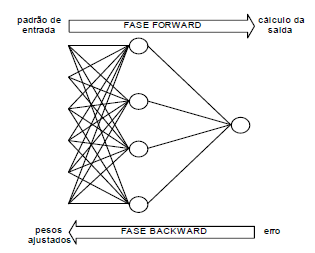
\includegraphics[width=0.65\textwidth]
             		{./Figs/08-mlp-back.png}
             	
             	\caption{Training phases of the MLP-Back-Propagation}.}\caption*{  Source:  \cite{Almeida2013}}\label{fig: MLP2}}
            \end{figure}
            
            In this method, as the error gradient is calculated from the lower to the upper layers, its norm decreases with exponential speed. This makes that in the layers closest to the entrance the weight adjustments are small, making the learning in them slower. This problem is known in the literature as \textit{vanishing gradient problem}. Usually the values of the learning rates stay between 0.2 and 0.8.
            
            In Neural Network training MLP with \textit{backpropagation}, validation only takes place with the stage of \textit{feedforward}, obtaining the quadratic errors of the output layer with the validation data observed. 
            
            As the ideal stopping point is a lower limit, the same is only discovered when it is exceeded after a few training periods, since in practical procedures the obtaining of an error is oscillatory and by which it is necessary to keep saved the parameters obtained during these periods.
            
            \paragraph{Weight readjustment optimizer} There are several algorithms known that optimize the convergence of the readjustment of the weights in the training of \textit{backpropagation}, uch as those mentioned below. The 'Momentum' optimizer speeds up the readjustment of the weights in search of minimum global errors, and 'RMSProp' prevents the search in the direction of oscillations. A third optimizer, called 'Adam' for the abbreviation 'Adaptive Moment optimization', combines these two characteristics. For the 'ADAM' algorithm, the learning rate can be arbitrated but in\citeonline{MLM} it is mentioned that a constant with a value of 0.001 has produced positive results in prediction problems.   
            
            In the figure \ref{fig:otimizadores} is compared the behavior of some optimizers. In this figure it is possible to see that the lower the cost of training, the greater the speed of convergence to the ideal readjustment of weights. Also, it is noticeable the computational advantage of 'ADAM' compared to other optimizers when increasing the number of iterations.
            
            \begin{figure}[ht]
            \center{
            	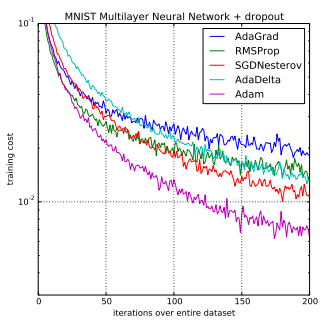
\includegraphics[width=0.70\textwidth]
            	{./Figuras/MLM/optimizers.png}
            
            \caption{Behavior of optimizers for MLP trained with \textit{Backpropagation}.}\caption*{  Source: \cite{MLM} }    \label{fig:otimizadores}}
        
            \end{figure}
            
    \subsection{Recurring Networks: The GRU model}\label{sec:GRU}

    The networks GRU, abbreviation of \textit{Gated Recurrent Unit},were first introduced in \cite{gru},being an adaptation of LSTM networks (Long Short-Term Memory).
    
    The LSTM networks were presented in \cite{lstm}, and use memory blocks called cells, which allow certain information to be kept on the network. The manipulation of information is made by \textit{gates} (by which the procedure is often called \textit{gating}). For these networks, there are three types of gates: i) forgetting gate, to remove information that is no longer useful, ii) input gate, to add useful information to the cell condition, and iii) output gate, to extract useful information from the cell condition. 
    
    LSTM networks allowed the resolution of more complex problems, but still had the problem of dissipating the gradient by which the memory could not maintain information of long sequences using the term of short-term memory.
    
    The GRU recurring networks solved this problem by changing the use of cell state to a hidden state with two new gates. These gates, called \textit{update gate} and \textit{reset gate} determine which information should be passed to the output and can be trained to maintain long sequence information without being dissipated of the values. 
    
    In \cite{DLB}, these gates are cited as the useful structures for solving prediction problems. In the Figure \ref{fig:gru-arch} are presented two network models, an LSTM and a GRU, indicating the gates in each one. 
         	
    \begin{figure}[ht]
    	\center{
    		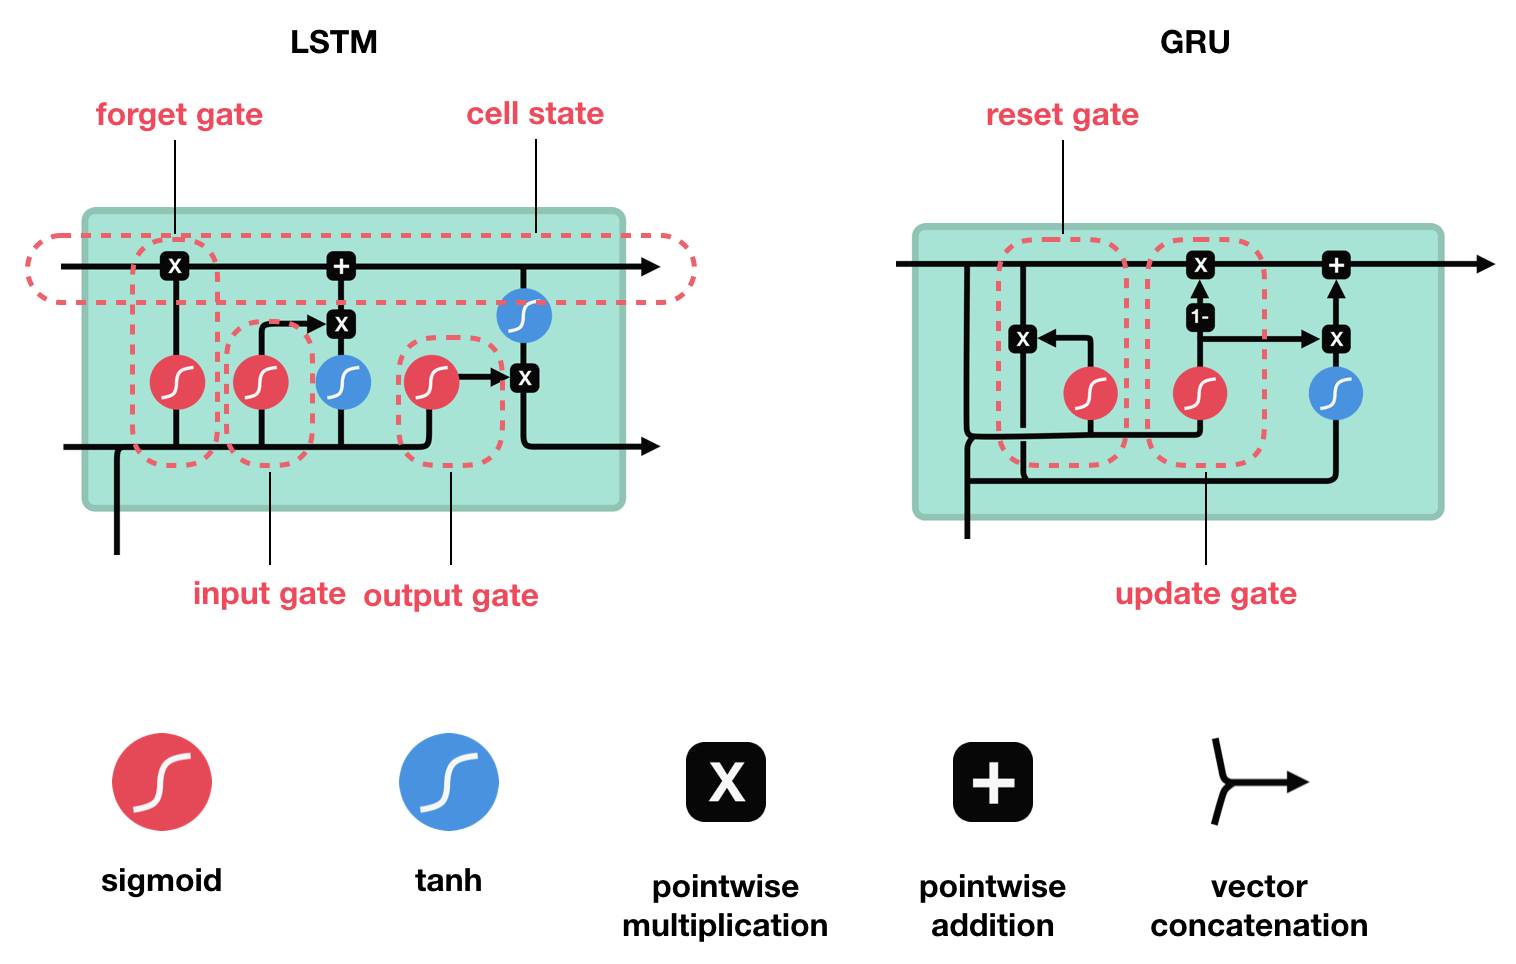
\includegraphics[width=0.80\textwidth]
    		{./Figs/10-portoes-rnns.png}
    	 	\caption{Architecture of the GRU model.}\caption*{  Source: \cite{DLB}} \label{fig:gru-arch}}
    \end{figure}
    
    The GRU networks then allowed the solution of problems with long sequences of data, solving the problem of short-term memory. So the biggest difficulty that could still arise in supervised trials was due to overfitting, by which another tool was proposed to prevent the network from memorizing beyond what was desired: the method \textit{dropout}.
    
    \subsubsection{Dropout} \label{sec:drop_fund}
    
    The \textit{Dropout} method has been introduced in \cite{dropout}, a term translated into Portuguese in the literature as abandonment, and proposes the temporary removal of some cell from the network. 
    
    In \cite{dropoutapp} has been applied \textit{dropout} was applied in the training of a neural net, in which, in each training period some cells of the entry layer are randomly disconnected and some of the hidden layers are all reconnected at the end of the training period. Thus, in each training season only a sample of the data is processed by a subset of the hidden cells.  
    
    This method seeks that the randomness of the choice of cells in each period induces a reduction in the dependence between them in the process of adjustment, making each unit generate patterns that do not depend on those learned by others. At the time of the test, all weights are multiplied by the probability that your cell has been turned off. 
    
    In \cite{dropoutapp} successful network training results are obtained with \textit{dropout} when in each season 50\% of the cells are disconnected in hidden layers and 20\% of the cells in the entrance layer.
    

    

